% !TEX TS-program = pdflatex
% !TEX encoding = UTF-8 Unicode

% This file is a template using the "beamer" package to create slides for a talk or presentation
% - Giving a talk on some subject.
% - The talk is between 15min and 45min long.
% - Style is ornate.

% MODIFIED by Jonathan Kew, 2008-07-06
% The header comments and encoding in this file were modified for inclusion with TeXworks.
% The content is otherwise unchanged from the original distributed with the beamer package.

\documentclass{beamer}
\setbeamercovered{invisible}



% Copyright 2004 by Till Tantau <tantau@users.sourceforge.net>.
%
% In principle, this file can be redistributed and/or modified under
% the terms of the GNU Public License, version 2.
%
% However, this file is supposed to be a template to be modified
% for your own needs. For this reason, if you use this file as a
% template and not specifically distribute it as part of a another
% package/program, I grant the extra permission to freely copy and
% modify this file as you see fit and even to delete this copyright
% notice. 


\mode<presentation>
{
  \usetheme{Warsaw}
  % or ...

  % or whatever (possibly just delete it)
}


\usepackage[english]{babel}
% or whatever

\usepackage[utf8]{inputenc}
% or whatever

\usepackage{times}
\usepackage[T1]{fontenc}
% Or whatever. Note that the encoding and the font should match. If T1
% does not look nice, try deleting the line with the fontenc.

%%% MATH RELATED


%%% AMS math stuff
\usepackage{amsmath}
\usepackage{amssymb}
\usepackage{amsthm}
\usepackage{mathrsfs}
\usepackage{enumerate}

%%% Theorem environments
\newtheorem{thm}{Theorem}[subsection]
\newtheorem{prop}[thm]{Proposition}
\newtheorem{cor}{Corollary}[thm]
\newtheorem{por}[thm]{Porism}
\newtheorem{lem}[thm]{Lemma}
\theoremstyle{definition}
\newtheorem{prob}[thm]{Problem}
\newtheorem{soln}{Solution}
\newtheorem{defn}[thm]{Definition}
\newtheorem{ex}[thm]{Example}
\newtheorem{quest}[thm]{Question}
\newtheorem{remk}[thm]{Remark}

%%% Typesetting shortcuts
\newcommand{\tn}[1]{\textnormal{#1}}
\newcommand{\ol}[1]{\overline{#1}}
\newcommand{\wt}[1]{\widetilde{#1}}
\newcommand{\wh}[1]{\widehat{#1}}
\newcommand{\vocab}[1]{\textbf{#1}\index{#1}}

%%% Math shortcuts
\newcommand{\bbr}{\mathbb R}
\newcommand{\bbz}{\mathbb Z}
\newcommand{\bbq}{\mathbb Q}
\newcommand{\bbn}{\mathbb N}
\newcommand{\bbf}{\mathbb F}
\newcommand{\bbc}{\mathbb C}
\newcommand{\bbd}{\mathbb D}
\newcommand{\bba}{\mathbb A}
\newcommand{\bbp}{\mathbb P}
\newcommand{\bbg}{\mathbb G}
\newcommand{\bbv}{\mathbb V}
\newcommand{\dih}[1]{\mathcal D_{#1}}
\newcommand{\sym}[1]{\mathcal S_{#1}}
\newcommand{\vspan}{\tn{span}}
\newcommand{\trace}{\tn{trace}}
\newcommand{\diff}{\backslash}
\newcommand{\stab}{\tn{stab}}
\newcommand{\conv}{\tn{conv}}
\newcommand{\img}{\tn{img}}
\newcommand{\coker}{\tn{coker}}
\newcommand{\id}{\tn{id}}
\newcommand{\Hom}{\tn{Hom}}
\newcommand{\End}{\tn{End}}
\newcommand{\Aut}{\tn{Aut}}
\newcommand{\aut}{\tn{Aut}}
\newcommand{\ann}{\tn{Ann}}
\newcommand{\GL}{\tn{GL}}
\newcommand{\Gr}{\tn{Gr}}
\newcommand{\lord}{\preccurlyeq}
\newcommand{\rord}{\succcurlyeq}
\newcommand{\tr}{\textnormal{Tr}}
\newcommand{\Tr}{\textnormal{Tr}}
\newcommand{\bbl}{\mathbb{L}}
\newcommand{\C}{\mathscr{C}}
\newcommand{\X}{\mathscr{X}}
\renewcommand{\S}{\mathscr{S}}
\newcommand{\M}{\mathscr{M}}
\renewcommand{\L}{\mathcal{L}}


%%% Algebraic Geometry
\newcommand{\height}{\textnormal{ht}}
\newcommand{\A}{\mathbb{A}}
\newcommand{\p}{\mathfrak{p}}
\newcommand{\sheaf}[1]{\mathcal{#1}}
\newcommand{\spec}{\textnormal{Spec}}
\newcommand{\proj}{\textnormal{Proj}}
\newcommand{\Aff}{\textnormal{Aff}}
\newcommand{\skel}{\textnormal{skel}}
\newcommand{\supp}{\textnormal{supp}}
\newcommand{\orb}{\textnormal{orb}}
\newcommand{\Proj}{\textnormal{Proj}}
\newcommand{\Pic}{\textnormal{Pic}}
\newcommand{\Rees}{\textnormal{Rees}}
\newcommand{\shom}{\mathcal{H}om}

\renewcommand*\arraystretch{1.3}

%%% paper specific definitions
\newcommand{\weyl}{\Omega}
\newcommand{\weyll}{{\widehat{\Omega}}}
\newcommand{\weylll}{{\widetilde{\Omega}}}
\newcommand{\mweyl}{{M_N(\Omega)}}
\newcommand{\mweyll}{{M_N(\widehat{\Omega})}}
\newcommand{\mweylll}{{M_N(\widetilde{\Omega})}}
\newcommand{\seq}{\text{Seq}}
\newcommand{\tail}{\text{Tail}}
\newcommand{\Ad}{\textnormal{Ad}}
\newcommand{\sech}{\textnormal{sech}}
\newcommand{\colim}{\varinjlim}
\newcommand{\limit}{\varprojlim}
\newcommand{\Bis}{\textnormal{Bis}}
\newcommand{\m}{\mathfrak{m}}
\newcommand{\mxx}[4]{\left(\begin{array}{cc} #1 & #2\\ #3 & #4 \end{array}\right)}
\newcommand{\diag}{\text{diag}}
\newcommand{\qdet}{\textnormal{qdet}}
\newcommand{\mdet}{\textnormal{mdet}}
\newcommand{\mtau}{\mathcal{T}}
\newcommand{\cof}{\textnormal{cof}}
\newcommand{\minor}{\textnormal{minor}}
\newcommand{\holo}{Holo}
\newcommand{\ord}{\textnormal{order}}
\newcommand{\mult}{\mathfrak M}






\title{MATH 350-2 Advanced Calculus} 
\subtitle
{} % (optional)

\author[W.R. Casper] % (optional, use only with lots of authors)
{W.R. Casper}
% - Use the \inst{?} command only if the authors have different
%   affiliation.

\institute[California State University Fullerton] % (optional, but mostly needed)
{
  Department of Mathematics\\
  California State University Fullerton}
% - Use the \inst command only if there are several affiliations.
% - Keep it simple, no one is interested in your street address.

\subject{Talks}
% This is only inserted into the PDF information catalog. Can be left
% out. 



% If you have a file called "university-logo-filename.xxx", where xxx
% is a graphic format that can be processed by latex or pdflatex,
% resp., then you can add a logo as follows:

% \pgfdeclareimage[height=0.5cm]{university-logo}{university-logo-filename}
% \logo{\pgfuseimage{university-logo}}



% Delete this, if you do not want the table of contents to pop up at
% the beginning of each subsection:
\AtBeginSubsection[]
{
  \begin{frame}<beamer>{Outline}
    \tableofcontents[currentsection,currentsubsection]
  \end{frame}
}


% If you wish to uncover everything in a step-wise fashion, uncomment
% the following command: 

%\beamerdefaultoverlayspecification{<+->}


\begin{document}

\begin{frame}
  \titlepage
\end{frame}

\begin{frame}{Outline}
  \tableofcontents
  % You might wish to add the option [pausesections]
\end{frame}

% Since this a solution template for a generic talk, very little can
% be said about how it should be structured. However, the talk length
% of between 15min and 45min and the theme suggest that you stick to
% the following rules:  

% - Exactly two or three sections (other than the summary).
% - At *most* three subsections per section.
% - Talk about 30s to 2min per frame. So there should be between about
%   15 and 30 frames, all told.

\section{Real Analysis Lecture 2}

\subsection{Types of real numbers}
\begin{frame}{Real numbers}
The \textbf{real numbers} are the unique field $\mathbb{R}$ satisfying Axiom 1-Axiom 9, plus an extra axiom called the completeness axiom.
$$\mathbb{R} = \text{the one and only complete, ordered field}$$
A complete ordered field $F$ satisfies
\begin{enumerate}[\text{A}1]
\setcounter{enumi}{5}
\pause
\item \textbf{completeness axiom}: every bounded set of numbers $S\subseteq F$ has a supremum $\sup(S)$
\end{enumerate}
\begin{itemize}
\pause
\item Understanding what this is challenging, but will be fundamental to the entire course!
\pause
\item Intuitively, it represents the fact that the real line has no holes or gaps.
\end{itemize}
\end{frame}


\begin{frame}{Real intervals}
Given an ordered field, we can \textbf{intervals}
\begin{itemize}
{\small
\pause
\item \textbf{open and closed intervals}
$$(a,b) = \{x\in \mathbb{R}: a < x < b\}
\quad\text{and}\quad
[a,b] = \{x\in \mathbb{R}: a \leq x \leq b\}$$
\pause
\item \textbf{half-open intervals}
$$
[a,b) = \{x\in \mathbb{R}: a \leq x < b\}
\quad\text{and}\quad
(a,b] = \{x\in \mathbb{R}: a < x \leq b\}
$$
\pause
\item \textbf{semi-infinite open intervals}
$$
(-\infty, a) = \{x\in\mathbb{R}: x < a\}
\quad\text{and}\quad
(a, \infty)  = \{x\in\mathbb{R}: a < x\}$$
\pause
\item \textbf{semi-infinite closed intervals}
$$
(-\infty, a] = \{x\in\mathbb{R}: x \leq a\}
\quad\text{and}\quad
[a, \infty)  = \{x\in\mathbb{R}: a \leq x\}.$$
}
\end{itemize}
\end{frame}

\subsection{Integers}

\begin{frame}{Inductive sets}
A subset $S$ of $\mathbb{R}$ is called a \vocab{inductive set} if
\begin{itemize}
\item $1\in S$
\item if $x\in S$ then $x+1\in S$ 
\end{itemize}
\pause
Examples:
$$\mathbb{R},\quad\mathbb{Q},\quad(0,\infty),\quad\mathbb{Z},\quad\mathbb{N},\dots$$
\end{frame}

\begin{frame}{Integers and rationals}
How do we reverse-engineer the integers from the reals?
\begin{itemize}
\pause
\item the set of \textbf{positive integers} is
$$\mathbb{Z}_+ = \{x: \text{$x$ belongs to every inductive set}\}$$
\pause
\item integers are
$$\mathbb{Z} = \{x: \text{$x$ is zero or $\pm x$ is a positive integer}\}$$
\pause
\item rationals are
$$\mathbb{Q} = \{a/b: a,b\in\mathbb{Z},\ b\neq 0\}.$$
\end{itemize}
\end{frame}

\begin{frame}{Induction}
\textbf{Principle of Induction:}
$$\text{If $S$ is an inductive set, then $\mathbb{Z}_+\subseteq S$}$$
\pause
\begin{quest}
Waaaaait...How is this this induction?!
\end{quest}
\pause
\textbf{Example:} Let's prove $n(n+1)$ is divisible by $2$ for all positive integers $n$, using the Principle of Induction.\\
\pause
\textbf{Proof:}\\
\pause
Let
$$S = \{n\in\mathbb{Z}_+: 2 | n(n+1)\}$$.
\pause
We see that $1\in S$ because $2$ divides $1(1+1)$.\\
\pause
Now suppose $x\in S$.  (This is our usual inductive assumption).\\
\end{frame}
\begin{frame}{Induction}
\textbf{Example:} Let's prove $n(n+1)$ is divisible by $2$ for all positive integers $n$, using the Principle of Induction.\\
\textbf{Proof continued:}\\
\pause
Then $2$ divides $x(x+1)$, so $x(x+1) = 2k$ for some integer $k$.\\
\pause
This means $(x+1)(x+2) = x(x+1) + 2(x+1) = 2(k+x+1)$.\\
\pause
Thus $2$ divides $(x+1)(x+2)$, showing that $x+1\in S$.\\
\pause
Since $x+1$ was arbitrary, this shows that $S$ is an inductive set.\\
\pause
By the Principle of Induction, this means $\mathbb{Z}_+\subseteq S$.\\
\pause
In other words $n\in S$ for every positive integer $n$.\\
\pause
Hence $2$ divides $n(n+1)$ for every positive integers $n$.
\end{frame}


\begin{frame}{Prime numbers}
A positive integer $p$ is \textbf{prime} if its only positive divisors are $1$ and $p$.
\begin{thm}[Apostol Theorem 1.5]
Every integer is prime or a product of primes
\end{thm}
\begin{thm}[Apostol Theorem 1.8]
If $p$ is prime and $p$ divides $ab$, then $p$ divides $a$ or $p$ divides $b$.
\end{thm}
\begin{thm}[Fundamental Theorem of Arithmetic (Apostol Theorem 1.9)]
Every integer $n > 1$ has a unique factorization as a product of primes, up to reordering.
\end{thm}

\end{frame}


\begin{frame}{Types of numbers}
\begin{center}
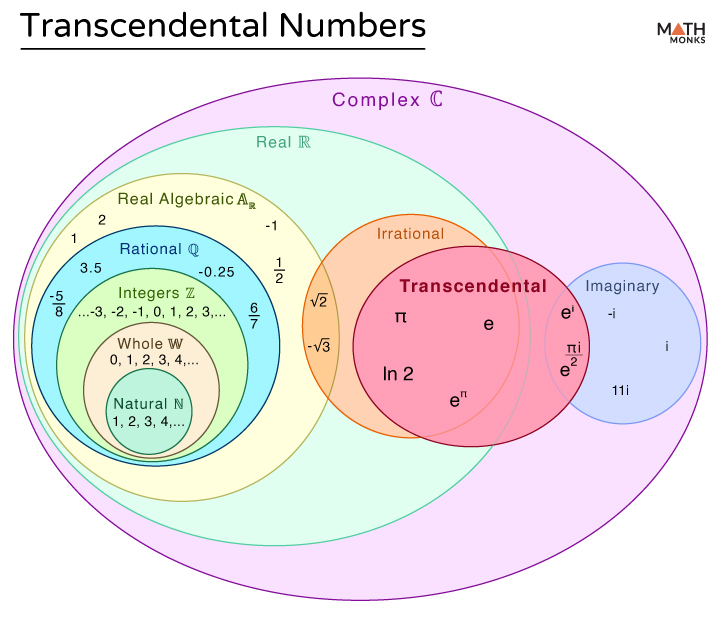
\includegraphics[width=0.8\linewidth]{fig/numbers}
\end{center}
\end{frame}

\begin{frame}{Irrational numbers}
Numbers which are not of the form $a/b$ with $a,b\in\mathbb{Z}$ are called \vocab{irrational}.\\
\begin{itemize}
\item Discovered by Hippasus, a pythagorean (a student of Pythagoras)
\end{itemize}
\begin{center}
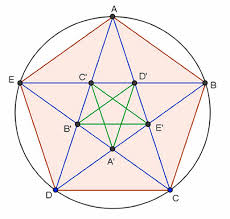
\includegraphics[width=0.4\linewidth]{fig/pentagram}
\end{center}
\end{frame}

\begin{frame}{Irrational numbers}
Numbers which are not of the form $a/b$ with $a,b\in\mathbb{Z}$ are called \vocab{irrational}.\\
\begin{itemize}
\item Pythagoras drowned Hippasus at sea for his discovery
\pause
\item dramatic reenactment, found online:
\pause
\end{itemize}
\pause
\begin{center}
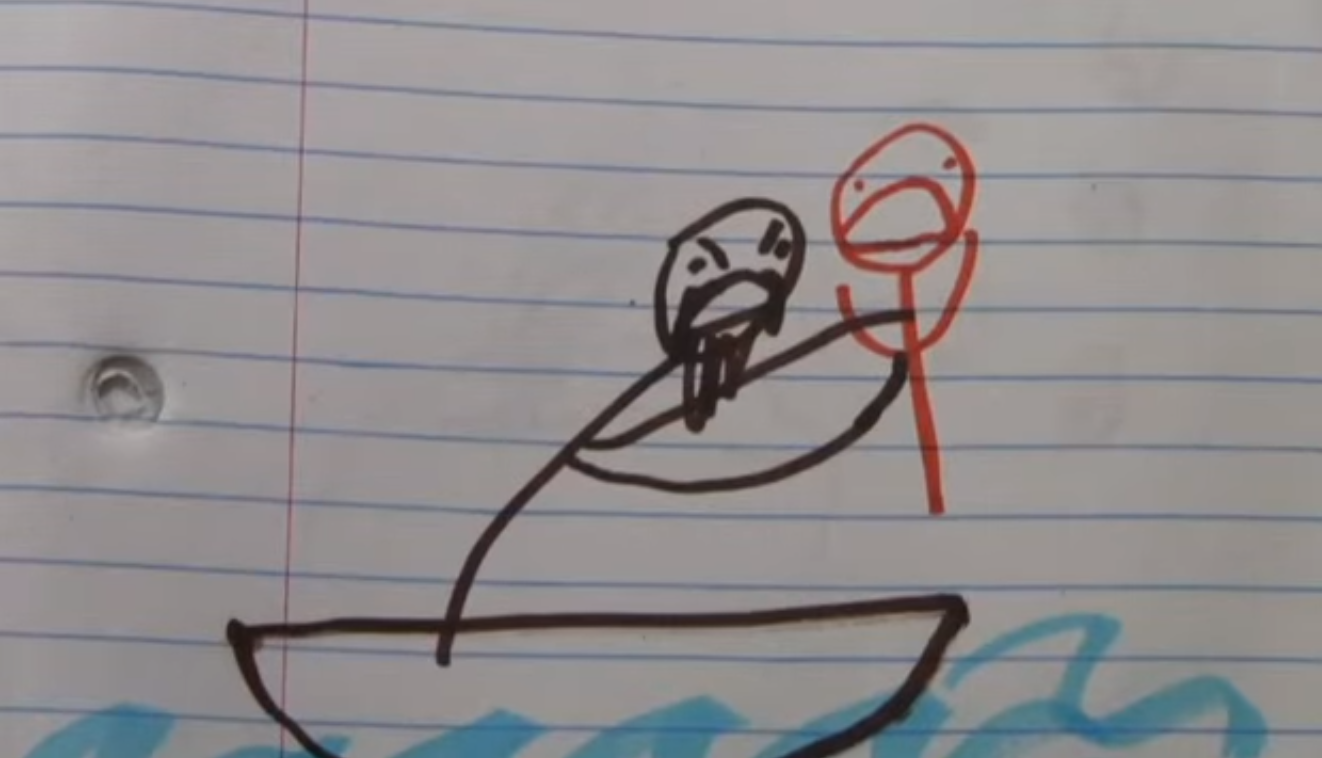
\includegraphics[width=0.6\linewidth]{fig/hippasus-death}
\end{center}
\end{frame}

\begin{frame}{Irrational numbers}
Numbers which are not of the form $a/b$ with $a,b\in\mathbb{Z}$ are called \vocab{irrational}.\\
\begin{itemize}
\item Pythagoras drowned Hippasus at sea for his discovery
\item anime style:
\pause
\end{itemize}
\begin{center}

\includegraphics[width=0.4\linewidth]{fig/jojo-hippasus}
\end{center}
\end{frame}

\begin{frame}{Challenge!}
\begin{prob}
Can you prove that if $n\in\mathbb{Z}_+$ is not a perfect square, then $\sqrt{n}$ is irrationial?
(Apostol Theorem 1.10)
\end{prob}
\pause
\begin{soln}
We prove by contradiction. \pause
Assume $\sqrt{n} = a/b$ for integers $a,b$. \pause
Without loss of generality, we may assume $\gcd(a,b) = 1$. \pause
Then $b^2n = a^2$. \pause
Since $\gcd(a,b) = 1$, $a^2$ must divide $n$, ie. $n=n'a^2$. \pause
It follows that $b^2n' = 1$, so $b^2$ divides $1$. \pause
This implies $n'$ divides $1$, so $n'=\pm 1$. \pause
Since $n>0$, $n'>0$ so $n'=1$. \pause
Thus $n=a^2$, which is a contradiction.
\end{soln}
\end{frame}

\begin{frame}{Algebraic and Transcendental}
Irrational numbers can be further divided into to categories
\pause
\begin{enumerate}
\item \textbf{algebraic numbers:} numbers which are roots of polynomials with integer coefficients, like
$$\sqrt{2},\quad\sqrt{3},\quad\text{and}\quad\sqrt[3]{\sqrt{5}  + \sqrt{7}}.$$
\pause
\item \textbf{transcendental numbers:} numbers which are not algebraic, like
$$\pi,\quad e,\quad e^\pi,\quad\text{and maybe}\quad\pi+e?$$
\pause
\item transcendentals are mysterious ... but most real numbers are transcendental!
\end{enumerate}
\end{frame}

\subsection{Upper Bound and Supremum}

\begin{frame}{Upper bounds}
An \textbf{upper bound} for a set $S\subseteq\mathbb{R}$ is a number $b$ such that
$$x \leq b\quad\text{for all}\ x\in S.$$
\pause
In this case, we say $S$ is \textbf{bounded above} by $b$.\\
\pause
If $b\in S$ also, then $b$ is called a \textbf{maximal element} of $S$
\pause
\textbf{Examples:}
\begin{itemize}
\pause
\item $34$ is an upper bound of $[-1,5]$, but not a maximal element
\pause
\item $5$ is a maximal element of $[-1,5]$
\pause
\item $3$ is an upper bound of $[0,3)$, but not a maximal element
\pause
\item $\mathbb{Z}_+$ has no upper bound
\pause
\item $[3,7)$ has an upper bound but no maximal element
\end{itemize}
\end{frame}


\begin{frame}{Challenge!}
\begin{prob}
Show that if $S$ has a maximal element, then it is unique.
\end{prob}
\pause
\textbf{Hint: use the definition!}
\pause
\begin{soln}
Suppose that $b_1$ and $b_2$ are both maximal elements of $S$.\\
\pause
Then $x\leq b_1$ and $x\leq b_2$ for all $x\in S$.\\
\pause
Moreover, $b_1\in S$ and $b_2\in S$.\\
\pause
Since $b_1\in S$ and $b_2$ is an upper bound of $S$, $b_1\leq b_2$.\\
\pause
Likewise, since $b_2\in S$ and $b_1$ is an upper bound of $S$, $b_2\leq b_1$.\\
\pause
By the trichotomy, we find $b_1=b_2$.
\end{soln}
\pause
Now we can say \emph{the} maximum, $\max(S)$
\end{frame}

\begin{frame}{Supremum}
A \textbf{supremum} of a set $S$ of real numbers is a real number $b\in\mathbb{R}$ such that
\begin{itemize}
\item $b$ is an upper bound of $S$
\item if $b'<b$, then $b'$ is not an upper bound of $S$
\end{itemize}
\pause
In other words
$$\text{a supremum is a \bf{least upper bound}}$$
\end{frame}

\begin{frame}{Challenge!}
\begin{prob}
Show that if $S$ has a supremum, then it is unique.
\end{prob}
\pause
\textbf{Hint: use the definition!}
\pause
\begin{soln}
Suppose that $b_1$ and $b_2$ are both suprema of $S$.\\
\pause
Then $b_1$ and $b_2$ are both upper bounds of $S$.\\
\pause
Since $b_1$ is a least upper bound, $b_1\leq b_2$.\\
\pause
Since $b_2$ is also a least upper bound, $b_2\leq b_1$.\\
\pause
By the trichotomy, we find $b_1=b_2$.
\end{soln}
\pause
Now we can say \emph{the} supremum, $\sup(S)$
\end{frame}

\begin{frame}{Challenge!}
\begin{prob}
Show that if $S$ has a maximum element.  Then $S$ has a supremum and $\max(S)=\sup(S)$
\end{prob}
\pause
\textbf{Hint: use the definition!}
\pause
\begin{soln}
Let $b=\max(S)$.\\
\pause
Then $b$ is an upper bound of $S$ and $b\in S$.\\
\pause
If $b'$ is another upper bound of $S$, then by definition $b\leq b'$.\\
\pause
Thus $b$ is the least upper bound of $S$.
\end{soln}
\end{frame}

\begin{frame}{Completeness Axiom}
Now we have the machinery in place to state the Completeness Axiom.
\pause
\begin{enumerate}[\text{A}1]
\setcounter{enumi}{9}
\pause
\item \textbf{completeness axiom}: if $S$ is any subset of real numbers which is bounded above, then it has a supremum $\sup(S)$
\end{enumerate}
\pause
\textbf{Examples:}
\begin{itemize}
\pause
\item $3$ is the supremum of $(0,3)$
\pause
\item $1$ is the supremum of
$$\left\lbrace
\frac{n}{n+1}: n\in\mathbb{Z}_+
\right\rbrace$$
\pause
\item $\pi$ is the supremum of
$$\{3,3.1,3.14,3.141,3.1415,3.14159,3.141592,\dots\}.$$
\end{itemize}
\end{frame}


\end{document}
